\begin{table}[htpb]
    \centering
    \caption{Some short unfamiliar terminologies in Neural Network}
    {\footnotesize

}
    {\small
    \begin{tabular}{cp{32em}}
        \toprule
        Terminology & Explanations \\
        \midrule
        \textbf{Seq2Vec with attention} & for text classification, attention identifies the relevant parts of the input. \\
        \textbf{self-attention} & $\bm{y}_i=\mathrm{Attn}(\mathbf{W}_q^e\bm{x}_i,(\mathbf{W}_k^e\bm{x}_1,\mathbf{W}_v^e\bm{x}_1),\cdots,(\mathbf{W}_k^e\bm{x}_n,\mathbf{W}_v^e\bm{x}_n))$ (encoder) \\
        \textbf{masked attention} & $\bm{y}_i=\mathrm{Attn}(\mathbf{W}_q^d\bm{y}_{i-1},(\mathbf{W}_k^d\bm{y}_1,\mathbf{W}_v^d\bm{y}_1),\cdots,(\mathbf{W}_k^d\bm{y}_{\color{red}i-1},\mathbf{W}_v^d\bm{y}_{\color{red}i-1}))$ (decoder when inference), similar with causal 1D CNN \\
        \textbf{multi-headed attention} & There are a set of $\mathbf{W}_{q_i}$, $\mathbf{W}_{k_i}$, and $\mathbf{W}_{v_i}$ to capture multiple set of features in parallel and \textit{fuse them to a single one} by $\mathbf{W}_o\in\mathbb{R}^{p_o\times hp_v}$.\\
        \textbf{positional encoding} & $\mathbf{X}+\mathbf{P}$, usually use a sinusoidal basis $p_{i,2j}=\sin\left(\frac{i}{C^{2j/d}}\right)$, $p_{i,2j+1}=\cos\left(\frac{i}{C^{2j/d}}\right)$, $i=1:T$ and $d$ is determined by the embedding dimension. PE is similar with binary code of position integers but \textit{more compact}.\\
        \textbf{ViT} & Vision Transformer, split a image to a sequence of $16\times 16$ patches and feed them (prepended a learnable patches, may act as an intercept \uline{representing the whole image like CLS in sequence}) into a transformer encoder for further embedding and classification\\
        \textbf{ELMo} & Embeddings from Language Model, context-specific embedding of each token, $\bm{r}_t^j=\bm{r}_t^\mathsf{T}\bm{w}^j$, 
        where $\bm{r}_t$ is the concatenation of all context and hidden vectors in a RNN model trained in an unsupervised way 
        and $t\to $ lower layer if syntactic task or $t\to$ higher layer if  semantic task \\
        \textbf{masked language model task} &  compute the loss at the masked locations given the others. \\
        \textbf{next sentence prediction task} & For a seq-pair $[\mathrm{CLS}~A_1~A_2\cdots A_m;~\mathrm{SEP}~B_1~B_2\cdots B_n~\mathrm{SEP}]$, 
        $y=1$ if $\mathbf{B}$ is the successor of $\mathbf{A}$ in original text else $y=0$. \\
        \textbf{TL;DR} & ``too long; didn't read'', token telling the model the user wants a summary. \\
        \textbf{T5} & ``Text-to-text Transfer Transformer'', a single model for multiple tasks 
        by telling the system what task to perform as part of the input sentence and then training it as a seq2seq model. \\
        \textbf{C4} & ``Colossal Clean Crawled Corpus'', a 750G corpus of web text for unsupervised training of T5. \\
        \textbf{locality sensitive hashing} & Two data points close in the original space will be close in the projected space by hashing in high probability otherwise in low probability. \\
        \bottomrule
    \end{tabular}}
    \label{tab:nn4imgseq}
\end{table}


\textbf{Attention mechanisms}: 
given $m$ \textbf{key}-\textbf{value} pairs $\{(\bm{k}_i\in\mathbb{R}^k,\bm{v}_i\in\mathbb{R}^v)\}_{i=1}^m$ (examplars) and 
an \textbf{query} $\bm{q}\in\mathbb{R}^q$ as input (new data point), some similarity between the query and keys is calculated 
as  
\begin{enumerate}[{(1)}]
    \item the \textit{weights} that linearly combine the corresponding values (soft attention)\unsure{
    Usually the dimensions of key and query ($k$ and $q$) are the same or mapped to a shared space and 
    $a$ can be any similarity measure $a:\mathbb{R}^{k\times q}\to\mathbb{R}$, 
    including parametric and non-parametric ones, 
    such as kernel functions $a(\bm{q},\bm{k}_i)=\mathcal{K}(\bm{q}-\bm{k}_i)$.
    }
    \begin{gather}
        \mathrm{Atten}(\bm{q},(\bm{k}_{1:m},\bm{v}_{1:m}))
        = \sum_{i=1}^m\alpha_i(\bm{q},\bm{k}_{1:m})=\sum_{i=1}^m\alpha_i(\bm{q},\bm{k}_{1:m})\bm{v}_i\in\mathbb{R}^v \\
        \alpha_i(\bm{q},\bm{k}_{1:m})
        = \mathrm{softmax}_i([{\color{purple}a}(\bm{q},\bm{k}_1),\cdots,{\color{purple}a}(\bm{q},\bm{k}_m)])
    \end{gather}
    \begin{enumerate}
        \item \textbf{additive attention}: 
        $a(\bm{q},\bm{k})=\bm{w}_v^\mathsf{T}\mathrm{tanh}(\mathbf{W}_q\bm{q}+\mathbf{W}_k\bm{k})\in\mathbb{R}$
        \item \textbf{dot-product attention}:\unsure{
        This type of attention is also applied to \textit{self-attention} in Transformer introduced later.
        }
        $a(\bm{q},\bm{k})=\bm{q}^\mathsf{T}\bm{k}/\sqrt{d}\in\mathbb{R}$\unsure{The denominator $\sqrt{q}$  is brought by the assumption of unit variance for $\bm{q}$ and $\bm{k}$.
        }
        \begin{gather}
            \Rightarrow \mathrm{Attn}(\mathbf{Q},]\mathbf{K},\mathbf{V})=\mathrm{softmax}(\frac{\mathbf{QK}^\mathsf{T}}{\sqrt{d}})\mathbf{V}\in\mathbb{R}^{n\times v}
        \end{gather}
    \end{enumerate}
    \item or extract the corresponding value with the \textit{maximal weight} (hard attention)
\end{enumerate}
to form a value fetched by the query.
The attention operation can be parallelized by padding a batch of jagged sequences
and then assigning a large negative value (usually $-10^6$ in practice) to the result of corresponding similarities,
which will generate a tiny weight by softmax to ``mask'' it.\unsure{
This masking mechanism can also be applied to any subset of a sequence, such as the future words after current query.
}

\textbf{Seq2Seq with attention}: allow the output words to directly ``look at'' the input words to avoid bottleneck that limits the information maintaining and to infer the alignment between source and target by calculating a \textit{dynamic context} $\bm{c}_t$ for each word in decoder.
\begin{gather}
    \bm{c}_t=\sum_{i=1}^T\underbrace{\alpha_i(\bm{h}_{t-1}^\mathrm{d},\bm{h}_{1:T}^\mathrm{e})}_{\text{weight},~\in\mathbb{R}}\bm{h}_i^\mathrm{e},\\
    \bm{h}_t^\mathrm{d}=f(\bm{h}_{t-1}^\mathrm{d},[\bm{y}_{t-1},\bm{c}_t])
\end{gather}

\textbf{(Seq+Seq)2Vec}: text pair classification (predicting the relationship between two sentences), 
\begin{enumerate}[{(i)}]
    \item translate seq1 and seq2 to the lengths of each other, 
    \item concatenate and fuse the original sequence features with that of the other's ``shadow'',
    \item pool the words of a fused sentence by summing to form context vector of a seq and its counterpart,
    \item concatenate the two context vectors and classify the relationship.
\end{enumerate}

\begin{figure}[htpb]
    \centering
    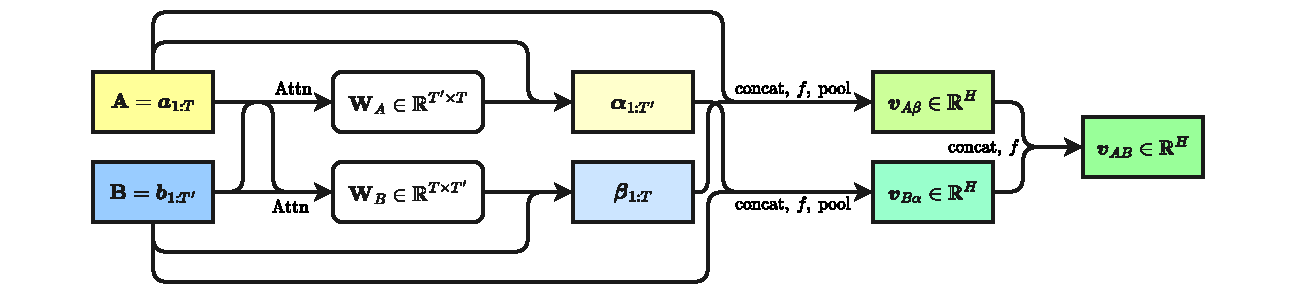
\includegraphics[width=0.9\textwidth]{figs/seqseq2vec.pdf}
    \caption{(Seq+Seq)2Vec}
    \label{fig:seqseq2vec}
\end{figure}


\textbf{Efficient transformers}: 
since the computational complexity of vanilla self-attention model is $O(n^2d)$, 
quadraticly increased with the length of sequence, the modification includes
\begin{enumerate}[{(1)}]
    \item \uline{fixed non-learnable localized attention patterns}: constrain the attention to a fixed non-learnable localized window (block, strided, dilated, or hybrid).
    \item \uline{learnable sparse attention patterns}: partition the long sequence by \textit{(locality sensitive) hashing} (Reformer) or \textit{clustering} (K-means).
    %\unsure{\color{red}I decided to skip it for now, and study it after finish reading this book. it is the famous \textbf{Reformer}'s idea, but I do not understand it yet...}
    \item \uline{memory sharing}: multiple tokens share a side memory module.
    \item \uline{recurrence}: connect different local blocks via recurrence.
    \item \uline{low-rank attention}: approximate attention using low rank matrices.
    \item \uline{kernel methods}: compute attention by kernel function (from low rank matrices), e.g. \textbf{Performer}\unsure{
    This model was considered to reduce PepNN's memory requirement, 
    but that time we did not implement it successfully.
    Its idea involves kernel method, and the details will refer to the following notes of Chapter 17.
    }
\end{enumerate}


\begin{example}
    \textbf{Performer}: Approximate the attention matrices by the kernel of random features

    Before normalization, the attention matrix $\mathbf{A}=[A_{ij}]\in\mathbb{R}^{N\times N}$ can be written as 
    \begin{gather}
        A_{ij}=\exp(\frac{\bm{q}_i^\mathsf{T}\bm{k}_j}{\sqrt{D}})
        = \underbrace{\exp(\frac{-\|\bm{q}_i-\bm{k}_j\|_2^2}{2\sqrt{D}})}_{\color{blue}\mathcal{K}_\text{gauss}(\bm{q}_i/D^{\frac{1}{4}},\bm{k}_j/D^{\frac{1}{4}})}
        \underbrace{\times \exp(\frac{\|\bm{q}_i\|_2^2}{2\sqrt{D}})
        \times \exp(\frac{\|\bm{k}_j\|_2^2}{2\sqrt{D}})}_\text{independent scaling factors}
    \end{gather}
    Moreover, the Gaussian kernel can be written as the expectation of a set of random features, which decouples $\bm{q}$ and $\bm{k}$:
    \begin{gather}
        \mathcal{K}_\text{gauss}(\bm{x},\bm{y})
        = \mathbb{E}\left[\bm{\eta}(\bm{x})^\mathsf{T}\bm{\eta}(\bm{y})\right]
    \end{gather}
    where the $\bm{\eta}(\bm{x})\in\mathbb{R}^M$ is based on trigonometric functions or \uline{exponential functions} 
    (with positive features and better results).
    Then the attention matrix can be rewritten as the following and estimated by a single sample of $\mathbf{Q}'$ and $\mathbf{K}'$
    \begin{gather}
        A_{ij}=\mathbb{E}\left[\bm{\phi}(\bm{q}_i)^\mathsf{T}\bm{\phi}(\bm{k}_j)\right] \\
        \bm{\phi}(\bm{x})\triangleq\exp(\frac{\|\bm{x}\|_2^2}{2\sqrt{D}})\bm{\eta}(\frac{\bm{x}}{D^\frac{1}{4}}) \\
        \Rightarrow
        \mathbf{A}=\mathbb{E}\left[\mathbf{Q}'(\mathbf{K}')^\mathsf{T}\right](\approx\mathbf{Q}'(\mathbf{K}')^\mathsf{T}=:\hat{\mathbf{A}}) \\
        \Rightarrow
        \hat{\mathrm{Attn}}(\mathbf{Q},\mathbf{K},\mathbf{V})=\mathrm{diag}^{-1}(\mathbf{Q}'[(\mathbf{K}')^\mathsf{T}\mathbf{1}_N])(\mathbf{Q}'{\color{blue}[(\mathbf{K}')^\mathsf{T}\mathbf{V}]})
    \end{gather}
    This decoupling of attention matrix enables the parallelization and reduce the memory requirement.
\end{example}

\begin{figure}[htpb]
    \centering
    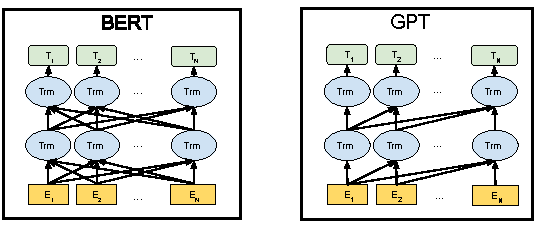
\includegraphics[width=0.8\textwidth]{figs/bertgpt.pdf}
    \caption{BERT \& GPT}
    {\footnotesize
    \textbf{BERT}: Bidirectional Encoder Representations from Transformers, used to create \textit{representations} of text;
    \textbf{GPT}: Generative Pre-training Transformer, used to \textit{generate} text.
    Their difference is whether the training is causal mode.
    }
    \label{fig:bertgpt}
\end{figure}


\section{Nonparametric Models}

\begin{table}[htpb]
    \centering
    \caption{Some short unfamiliar terminologies in Nonparametric Models}
    {\footnotesize

}
    {\small
    \begin{tabular}{cp{32em}}
        \toprule
        Terminology & Explanations \\
        \midrule
        \textbf{exemplar-based models} & \textbf{instance-based learning} and \textbf{memory-based learning}, keeping the training examples around at test times. \\
        \textbf{the curse of dimensionality} & \textit{empty high-dimensional universes that make you feel lonely} \\
        \textbf{k-d tree} & divides space into axis-parallel regions \\
        \textbf{open set recognition} & test samples may come from new categories. \\
        \textbf{online learning} & incremental learning, life-long learning, or continual learning, 
        which often involves \textbf{novelty detection} and encounters \textbf{out-of-distribution (OOD)} and \textbf{few-shot classification} \\
        \textbf{OOD} & Detecting the new class from some entirely different kind of distribution with the previous ones \\
        \textbf{few-shot classification} & only get a few (sometimes just one) example of each class \\
        \textbf{deep metric learning} & learning an embedding of original features $\bm{x}$ by \textit{deep learning models} and computing distances in the embedding space.\\
        \textbf{spherical embedding constraint} & an batchwise regularization term, encouraging all the examples to have the same norm, like Equation (\ref{eq:sec}) \\
        \textbf{stationary kernels} &  kernels whose value only depends on the elementwise difference between the inputs, i.e. $\mathcal{K}(\bm{x},\bm{x}')=\mathcal{K}(\|\bm{x}-\bm{x}'\|)$.
        Instead, \textbf{non-stationary kernel} functions cannot be expressed as simply a function of the distance between their inputs, $\bm{x}-\bm{x}'$.\\
        \textbf{Ornstein-Uhlenbeck process} & $\nu=\frac{1}{2}$ in Matern kernel (Equation (\ref{eq:maternk})), 
        continuous but not differentiable, and hence very ``jagged'', describing the \textit{velocity of a particle undergoing Brownian motion}. \\
        \bottomrule
    \end{tabular}}
    \label{tab:nonparam}
\end{table}




\subsection{Exemplar-based Methods}

\textbf{KNN}: A new nput's label distribution is decided by its $K$ nearest neighbors defined by \textit{Mahalanobis distance}.\unsure{
{\color{red}(How to define the covariance matrix $\mathbf{M}$ given the new input?)} 
This is a topic, \textbf{learning distance metrics}, worth discussed below.
}
\begin{gather}
    p(y=c|\bm{x},\mathcal{D})=\frac{1}{K}\sum_{n\in\mathsf{N}_K(\bm{x},\mathcal{D})} \mathbb{I}(y_n=c) \label{eq:knn} \\
    d_\mathbf{M}(\bm{x},\bm{\mu})=\sqrt{(\bm{x}-\bm{\mu})^\mathsf{T}\mathbf{M}(\bm{x}-\bm{\mu})}.
\end{gather}
Searching the nearest neighbors is the bottleneck of speed and memory requirement, thus the approximation methods are adopted. 
Package \texttt{FAISS} collects a lot of ones.

The methods to \textit{learn} the mahalanobis matrix $\mathbf{M}$ or 
\uline{a linear mapping $\mathbf{W}$ such that $\mathbf{M}=\mathbf{W}^\mathsf{T}\mathbf{W}$}:
\begin{enumerate}[{(1)}]
    \item \textbf{large margin nearest neighbor} (LMNN): in the training process, minimize the distances with the target neighbors with the same class label 
    (\textit{pull} the kindred to neighborhood), 
    and ensure the points with different class labels are more far away than any target neighbors 
    (\textit{push} away the imposters to a further place than the kindred)
    \begin{align}
        \mathcal{L}_\text{pull}(\mathbf{M})
        =&~ \sum_{i=1}^N\sum_{j\in\mathcal{N}_i}d_\mathbf{M}(\bm{x}_i,\bm{x}_j)^2 \\
        \mathcal{L}_\text{push}(\mathbf{M})
        =&~ \sum_{i=1}^N\sum_{j\in\mathcal{N}_i}\sum_{l=1}^N\mathbb{I}(y_i\neq y_l)\left[{\color{blue}m}+d_\mathbf{M}(\bm{x}_i,\bm{x}_j)^2-d_\mathbf{M}(\bm{x}_i,\bm{x}_l)^2\right]_+ \label{eq:lmnnpush} \\
        \mathcal{L}(\mathbf{M}) =&~ (1-\lambda)\mathcal{L}_\text{pull}(\mathbf{M}) + \lambda\mathcal{L}_\text{push}(\mathbf{M}) \\
        \text{or}~\mathcal{L}'(\mathbf{W}) =&~ \mathcal{L}(\mathbf{M}),
    \end{align}
    \item \textbf{neighborhood component analysis} (NCA): 
    maximize the \textit{expected number of correctly classified examples} according for a 1NN classifier by  leave-one-out error.
    \begin{align}
        p_{ij}^\mathbf{W} =&~ \frac{\exp(-\|\mathbf{W}\bm{x}_i-\mathbf{W}\bm{x}_j\|_2^2)}{\sum_{l\neq i}\exp(-\|\mathbf{W}\bm{x}_i-\mathbf{W}\bm{x}_l\|_2^2)} \\
        \mathcal{L}(\mathbf{W}) =&~ 1 - \frac{1}{N}J(\mathbf{W}) = 1 - \frac{1}{N}\sum_{i=1}^N\sum_{j\neq i,y_j=y_i}p_{ij}^\mathbf{W}
    \end{align}
    \item \textbf{latent coincidence analysis} (LCA): maximize the log marginal likelihood of pair's labels $y_n$ 
    by defining the \textit{hierarchical distributions} of \textit{projection} (Gaussian) and \textit{pair's labels} (Bernoulli) and \textit{EM optimization}.
    For a pair of points, $\bm{x}$ and $\bm{x}'$, and the pair index $n$,
    \begin{align}
        p(\bm{z}|\bm{x}) =&~ \mathcal{N}(\bm{z}|\mathbf{W}\bm{x},\sigma^2\mathbf{I}) \\
        p(y=1|\bm{z},\bm{z}') =&~ \exp(-\frac{1}{2\kappa^2}\|\bm{z}-\bm{z}'\|) \\
        \ell(\mathbf{W}, \sigma^2, \kappa^2) =&~ \sum_{n}\log{p(y_n|\bm{x}_n,\bm{x}_n')}
    \end{align}
    \item \textbf{deep metric learning} (DML): learn the distance directly by learning an embedding to a lower dimensional but ``semantic'' space.
    \begin{gather}
        \bm{e} = f(\bm{x};\bm{\theta})\in\mathbb{R}^E,~\hat{\bm{e}} = \frac{\bm{e}}{\|\bm{e}\|_2} \label{eq:sec} \\
        \begin{cases}
        \text{distance} & d(\bm{x}_i,\bm{x}_j;\bm{\theta})^2 = \|\hat{\bm{e}}_i-\hat{\bm{e}}_j\|_2^2 \\
        \text{similarity} & s(\bm{x}_i,\bm{x}_j;\bm{\theta})^2 = \hat{\bm{e}}_i^\mathsf{T}\hat{\bm{e}}_j
        \end{cases}
        {\color{gray}\Rightarrow d^2 = 2-2s^2} \\
    \end{gather}
    \begin{itemize}
        \item \textit{classification losses}: use the loss for classification if the data have label\unsure{
        where the labels act as the indicator of similarity.
        }
        \item \uline{\textbf{ranking loss}}: ensure that similar\unsure{
        The similarity is not necessary to be defined by labels.
        } examples are closer than dissimilar examples:
        \textit{contrastive loss} ($O(N^2)$),\unsure{
        Recall the LMNN's Equation (\ref{eq:lmnnpush})
        } 
        \textit{triplet loss} ($O(N^2)$) and \textit{N-pair loss} ($O(N^3)$)\unsure{
        Note that the $N$ is nothing to do with the total number of instances but pairs used in the loss,
        such as the \textit{hard negatives}.
        }
        {\footnotesize
        \begin{gather}
            \begin{cases}
                \mathcal{L}(\bm{\theta};\bm{x}_i,\bm{x}_j) 
                = \mathbb{I}(y_i=y_j)d(\bm{\bm{x}_i,\bm{x}_j};\bm{\theta})^2
                + \mathbb{I}(y_i\neq y_j)\left[m-d(\bm{x}_i,\bm{x}_j)\right]^2_+ \\
                \mathcal{L}(\bm{\theta};\bm{x}_i,\bm{x}_i^+,\bm{x}_i^-)
                = \left[d(\bm{x}_i,\bm{x}_i^+;\bm{\theta})^2 - d(\bm{x}_i,\bm{x}_i^-;\bm{\theta})^2+m\right]_+ \\
                \mathcal{L}(\bm{\theta};\bm{x},\bm{x}^+,\{\bm{x}_k^-\}_{k=1}^{N-1}) 
                = \log\left(1+\left[\sum_{k=1}^{N-1}\exp(s(\bm{x},\bm{x}_k^-;\bm{\theta}))\right] - s(\bm{x},\bm{x}^+;\bm{\theta})\right)
            \end{cases}
        \end{gather}
        }
    \end{itemize}
\end{enumerate}

The methods to speed up \textbf{ranking loss}'s optimization.
\begin{enumerate}[{(1)}]
    \item \uline{only consider \textit{hard negatives} or up to \textit{semi-hard negatives}}, which requires large batch size and whose set is updated during training. ($O(M^2)$ or $O(M^3)$, $M<N$)
    \item \uline{proxy methods}, measuring the distance between each anchor and \textit{a set of P proxies that represent each class} (updated during training), rather than directly measuring distance between examples. ($O(NP^2)$, $P\sim C<N$)
    \item {\color{gray}\uline{optimize an upper bound} (for the triplet loss) from \textit{triangle inequality} 
    with approximation gap $0\leq\mathcal{L}_t-\mathcal{L}_u\leq\frac{N^3}{C^2}K$, 
    where $K$ depends on the spread of the controids ($O(NC)$):\unsure{
    \color{red}Do not understand this method yet, reread it after finishing the weekly plan...
    }
    {\small\begin{align}
        \|\hat{\bm{e}}_i-\hat{\bm{e}}_j\|-\|\hat{\bm{e}}_i-\hat{\bm{e}}_k\|
        \triangleq&~ \ell_t(\bm{x}_i,\bm{x}_j,\bm{x}_k) \\
        \leq&~ \ell_u(\bm{x}_i,\bm{x}_j,\bm{x}_k) \\
        \triangleq&~ \|\hat{\bm{e}}_i-\bm{c}_{y_i}\|
        -\|\hat{\bm{e}}_i-\bm{c}_{y_k}\|
        +\|\hat{\bm{e}}_j-\bm{c}_{y_i}\|
        +\|\hat{\bm{e}}_j-\bm{c}_{y_k}\|
    \end{align}
    \begin{align}
        &\Rightarrow\sum_{(i,j)\in\mathcal{S},(i,k)\notin\mathcal{S}}\ell_t(\bm{x}_i,\bm{x}_j,\bm{x}_k)
        \triangleq \mathcal{L}_t(\mathcal{D},\mathcal{S}) 
        \leq \mathcal{L}_u(\mathcal{D},\mathcal{S}) \\
        &= \underbrace{3(C-1)(\frac{N}{C}-1)\frac{N}{C}}_{\text{const.}~C'}
        \sum_{i=1}^N\left(
            \|\bm{x}_i-\bm{c}_{y_i}\| - \frac{1}{3(C-1)}\sum_{m=1,m\neq y_i} \|\bm{x}_i-\bm{c}_m\|
        \right)
    \end{align}}}
\end{enumerate}

\textbf{Density kernel}: a function\unsure{
it can measure the similarity by converting from a distance. 
Actually \textit{any integrable function} satisfying 
(i) symmetry about 0, 
{\color{red}(ii) monotone decreasing in $\mathbb{R}^+$ (unimodal on 0)?} 
{\color{blue}It is not necessary, any covariance is possible. See the popular kernels and GP below}, and 
(iii) value $\to 0$ as $x\to\infty$ can serve as a density kernel by normalization.
} satisfying 
\begin{gather}
    \mathcal{K}:\mathbb{R}\to\mathbb{R}^+~\text{such that}~
    \begin{cases}
        \mathcal{K}(x)=\mathcal{K}(-x) & \text{\color{blue}(kernel)} \\
        \int{\mathcal{K}(x)}dx=1 & \text{\color{blue}(density)}
    \end{cases}\\
    \Rightarrow \int{x\mathcal{K}(x-x_n)}dx=x_n
\end{gather}\unsure{
Spread the effect of $x_n$ over the entire space with some covariance.
}
\begin{enumerate}[{(1)}]
    \item \uline{RBF kernel} (Gaussian kernel with bandwidth): $\frac{1}{h}\mathcal{N}(\frac{x}{h}|0,1)$.
    \footnote{To minimize the frequentist risk, set $h = \left(\prod_{d=1}^Dh_d\right)^{\frac{1}{D}}$, 
    where $h_d = \sigma_d\left(\frac{4}{3N}\right)^\frac{1}{5}$, $\hat{\sigma} = 1.4826\mathrm{MAD}$, 
    and $\mathrm{MAD} = \mathrm{median}(|\bm{x}-\mathrm{median}(\bm{x})|)$.}
    \item \uline{boxcar kernel}: $0.5\mathbb{I}(|x|\leq 1)$
    \item \uline{Epanechnikov kernel}: $\frac{3}{4}(1-x^2)\mathbb{I}(|x|\leq 1)$
    \item \uline{tri-{\color{red}cube} kernel}: $\frac{70}{81}(1-|x|^3)^{\color{red}3}\mathbb{I}(|x|\leq 1)$\unsure{
    with finite support and differentiable at supports and the boundaries.
    }
\end{enumerate}


\textbf{Kernel density estimation (KDE)}, a generative model, which defines a probability distribution $p(\bm{x})$
which can be evaluated pointwise and sampled from to generate new data.\unsure{
Recall the Gaussian mixture model with uniform class prior $p(\bm{x}|\bm{\theta})=\frac{1}{K}\sum_{k=1}^K\mathcal{N}(\bm{x}|\bm{\mu}_k,\sigma^2\mathbf{I})$, 
which can regarded as Gaussian kernel density ``estimation'' given $K$ ideal examplars $\bm{\mu}_k$.
}
\begin{gather}
    p(\bm{x}|\mathcal{D}) = \frac{1}{N}\sum_{n=1}^N\mathcal{K}(\bm{x}-\bm{x}_n)
\end{gather}

\textbf{Balloon kernel density estimator}: combine the idea of KNN and KNN, 
specify a dynamic bandwidth for KDE by growing a volume around new input $\bm{x}$ 
until encountering $K$ data points, regardless of their class label.
\begin{gather}
    p(\bm{x}|y=c,\mathcal{D})=\frac{N_c(\mathcal{V}_K(\bm{x}))}{|\mathcal{V}_K(\bm{x})|N_c(\mathcal{V}_\mathcal{D})}
\end{gather}
where $N_c(\mathcal{V})$ the number of examples with label $c$ in volume $\mathcal{V}$, 
$\mathcal{V}_K(\bm{x})$ the volume around $\bm{x}$ embracing $K$ examples, and
$\mathcal{V}_\mathcal{D}$ the entire data space. If the class prior $p(y=c)=\frac{N_c}{N}$,
then Balloon KDE is equivalent to KNN (Equation (\ref{eq:knn})).


\textbf{Kernel regression}:\unsure{
In attention mechanism, the similarity (pre-attention) scores are given by a \textit{non-parametric kernel function} 
and the \textit{values} are the \textit{examplars' labels}
}
In regression problem, do not cast parametric assumption of data distribution but estimate it by KDE, 
then it can show that the prediction is a weighted sum of outputs at the training points, 
where the weights depend on the similarity between the new input $\bm{x}$ and the corresponding training points.
\begin{align}
    \mathbb{E}[y|\bm{x},\mathcal{D}]
    =&~ \int{yp(y|\bm{x},\mathcal{D})}dy=\frac{\int{yp(\bm{x},y|\mathcal{D})}dy}{\int{p(\bm{x},y|\mathcal{D})}dy} \\
    p(\bm{x},y|\mathcal{D})
    \approx&~ \frac{1}{N}\sum_{n=1}^N\mathcal{K}_h(\bm{x}-\bm{x}_n)\mathcal{K}_h(y-y_n) \\
    \Rightarrow \mathbb{E}[y|\bm{x},\mathcal{D}]
    =&~\sum_{n=1}^N y_nw_n(\bm{x})\\
    w_n(\bm{x})
    \triangleq&~ \frac{\mathcal{K}_h(\bm{x}-\bm{x}_n)}{\sum_{n'=1}^N\mathcal{K}_h(\bm{x}-\bm{x}_{n'})}
\end{align}




\subsection{Kernel Methods}


\textbf{Mercer’s theorem}: $\forall$ kernel function $\mathcal{K}$ can be written as $\mathcal{K}(\bm{x},\bm{x}')=\bm{\phi}(\bm{x})^\mathsf{T}\bm{\phi}(\bm{x}')$,
where $\bm{\phi}(\cdot)$ is a feature extraction function that represent the original features $\bm{x}$ into a new feature space.
% (for positive definite matrix $\mathbf{K}$, $K_{ij}=[\mathbf{\Lambda}\frac{1}{2}\mathbf{U}_{:i}]^\mathsf{T}[\mathbf{\Lambda}\frac{1}{2}\mathbf{U}_{:j}]$)

Some popular kernel functions:\unsure{
kernel function describes the distribution of a series r.v. (new inputs) given a observation (anchor for a kernel function).
}
\begin{itemize}
    \item \textbf{automatic relevancy determination (ARD) kernel}: 
    If $d$ is an irrelevant input dimension, we can set $\ell_d = \infty$, 
    so the corresponding dimension will be ignored.
    \begin{gather}
        \mathcal{K}(\bm{r};\bm{\ell},\sigma^2)=\sigma^2\exp\left(
            -\frac{1}{2}\sum_{d=1}^D\frac{1}{\ell_d^2}r_d^2
        \right)
    \end{gather}

    \item \textbf{Matern kernel}: give rise to ``rougher'' functions,\unsure{
    Squared exponential (SE) kernels, $C\exp{(\|\cdot\|_2^2)}$, are infinitely differentiable.
    }
    which can better model local ``wiggles'' without having to make the overall length scale very small.
    \begin{gather}
        \mathcal{K}(r;\nu,\ell)=\frac{2^{1-\mu}}{\Gamma(\mu)}\left(
            \frac{\sqrt{2\mu r}}{\ell}
        \right)^\nu
        \underbrace{K_\nu\left(
            \frac{\sqrt{2\mu r}}{\ell}
        \right)}_\text{Bessel func.}\label{eq:maternk}
    \end{gather}
    
    \item \textbf{periodic kernel} and \textbf{cosine kernel}: capture repeating structure.
    \begin{gather}
        \mathcal{K}(r;\ell,p)=\exp\left(
            -\frac{2}{\ell^2}\sin^2(\pi\frac{r}{p})
        \right) \\
        \mathcal{K}(r;p)=\cos(2\pi\frac{r}{p})
    \end{gather}
    
    \item Old kernels can be \textit{transformed} or \textit{combined} by addition \& multiplication to a new one.
    
    \item \textbf{string kernel}: compare \textit{strings} in terms of the number of n-grams they have in common.
    
    \item \textbf{random walk kernel}: performs random walks on two\textit{graphs} simultaneously, 
    and then counts the number of paths that were produced by both walks.
\end{itemize}

